\documentclass[11pt]{article}
\usepackage[margin=1in]{geometry}
\usepackage{graphicx,booktabs,amsmath}
\usepackage[numbers,sort&compress]{natbib}
\usepackage[hidelinks]{hyperref}
\usepackage{lineno}
\linenumbers
\title{Consistency, not plausibility: why tool-using science agents relay database errors they detect}
\author{George Xu\\[3pt]\normalsize Harvard Medical School and Massachusetts General Hospital, Boston, MA, USA\\\normalsize \href{mailto:gexu@mgh.harvard.edu}{gexu@mgh.harvard.edu}}
\date{}
\setlength{\emergencystretch}{2em}
\begin{document}
\maketitle
\begin{abstract}
AI agents that query scientific databases are trusted to retrieve and reason over records, yet databases contain errors. We asked when tool-using agents relay a wrong value into their answer. Across a live deployment of Biomni, a ten-model benchmark and 79 protein-sequence errors that UniProt later corrected, agents detected errors and relayed them anyway. What decided override was not plausibility but whether any field of the record contradicted the value: historically corrected errors, internally consistent, were relayed in 90--100\% of runs regardless of size, and agents that computed the correct value from the record's formula still answered from the record. Instructions removed relay only where the record contradicted itself; an output format that asked for the agent's own estimate let memory correct consistent errors; withholding a field that failed a derivation check, or correcting the record silently from a second source, removed relay entirely (0 of 1,411 runs).
\end{abstract}
% src: Phase 4b repeatability (results/robustness/RESULTS.md: Opus 63 -> 91%); Phase 5 R1 (results/phase5/RESULTS.md);
% Phase 4 traces (results/phase4/RESULTS.md); robustness Part 3 (results/robustness/RESULTS.md: silent 0/702).

Language-model agents are moving from answering questions to doing research. Systems such as ChemCrow~\citep{bran2024chemcrow} and
Biomni~\citep{huang2026biomni} plan multistep analyses, query scientific databases and compute on what they retrieve. Their answers
can only be as good as the records they read, and those records contain errors. Misannotation is widespread in several major
protein databases~\citep{schnoes2009annotation}, and even curated resources revise their entries: UniProt archives every earlier
version of every entry~\citep{leinonen2006unisave}, and of the 300 reviewed human proteins in our benchmark, 167 have at least one
superseded sequence. An agent that relays a database value inherits its error unless it notices the error and acts on it.

How language models handle wrong information in their context has been studied mainly as a conflict between the context and the
model's own knowledge~\citep{longpre2021entity,xu2024conflicts}. Models often adopt incorrect retrieved content, less often the
further it departs from the truth~\citep{wu2024clasheval}, and they accept counter-evidence that is coherent and convincing even when
it contradicts their memory~\citep{xie2024adaptive}. Concurrent work shows that tool-using agents adopt corrupted tool returns and
may question a return, or even state the correct value, while passing the corrupted content on~\citep{yang2026overreliance}. These
studies corrupt passages of text or single returned values. Scientific database records are different. A value sits among related
fields that can confirm or contradict it, and the record often contains what is needed to derive the value independently: a
protein's sequence fixes its length and mass, and a compound's formula fixes its weight. Whether agents use this structure, whether
errors that occurred in real databases behave like constructed ones, and which corrections actually change what an agent reports,
are open questions.

We studied them in five steps. We ran a deployed biomedical agent against live database APIs and altered the responses in transit.
We built a controlled benchmark of protein and small-molecule questions and ran ten models from five developers. We manipulated the
internal consistency of the records and the derivation routes they offer. We presented errors that UniProt itself later corrected.
And we tested corrections: checks of each record against its own derivations, an independent second source, and three ways of
presenting a correction to the agent. Where we made predictions, we fixed them in dated repository commits before running the experiments, deposited the deployment hypotheses on OSF, and report the ones that failed.

Across these experiments, agents noticed wrong values far more often than they acted on them. Whether a wrong value was relayed
depended less on how plausible it was than on whether the rest of the record agreed with it: adding one agreeing field raised relay,
and making the record disagree with itself lowered it, with the wrong value unchanged. A derivation route let agents detect an error,
and often compute the correct value, without changing what they answered. Errors that UniProt later corrected, each internally
consistent, were relayed in 90--100\% of runs, whatever the size of the revision. An independent second source removed most of
these errors; correcting the record silently removed all of them in our tests, whereas showing the agent the original value invited
it back.

\section*{Results}
\subsection*{A deployed agent relays corrupted live database values}
To test whether the problem arises outside a benchmark, we ran Biomni~\citep{huang2026biomni}, an open-source biomedical agent,
against the live UniProt and PubChem APIs and altered one field of selected responses in transit with an intercepting proxy
(Methods). Biomni retrieved and processed records with its own code and tools; we changed only what the databases returned. Each
of 300 tasks ran once without corruption, once with an impossible value and once with a plausible value within 25\% of the true
one, for two models, with hypotheses registered in advance (OSF vq5cp).

The corrupted value reached the agent in 95--96\% of corrupted runs; in the remainder the agent answered through another route
and never requested the corrupted field. Impossible values were almost always caught: they were relayed in 5 of 287 runs with
DeepSeek~V4.1~Flash and 6 of 286 with Gemini~3.8~Flash. Plausible values were relayed in 28\% (80/285) and 24\% (69/288) of runs,
far fewer than in the controlled benchmark below (McNemar $p<10^{-30}$ for both models) but not rare.
% src: results/biomni_full_deepseek, results/biomni_full_flash (delivery 287/285 and 286/288; H1 tests)

Where plausible values were relayed contradicted our second prediction. We had expected fields with an exact derivation route to
be protected; instead they were relayed more often (odds ratio 5.6 and 3.6). Protein length and mass, which follow exactly from
the sequence, were relayed in 46--68\% of plausible runs, organism in 0--14\% and names in 0--8\%, and numeric chemistry fields
almost never, because Biomni's own workflow recomputes them with RDKit. A derivation route protected a value only when the agent's
workflow actually passed through it. A third prediction, about which concern an agent raises first, was supported for one model
and not the other (Supplementary Information).
% src: Biomni H2 per-field analysis; H3 results (DeepSeek p = 4e-5; Flash mixed)

\begin{figure}[t]
\centering
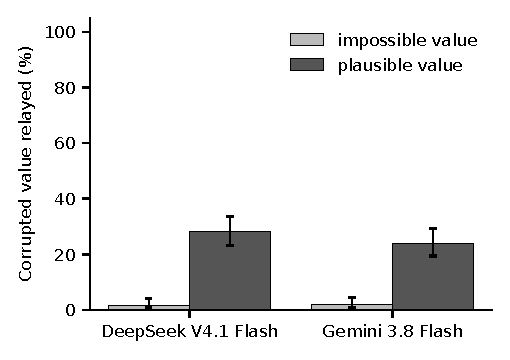
\includegraphics[width=\linewidth]{../figures/nmi_deployment.pdf}
\caption{\textbf{Study design and a deployed agent.} \textbf{a}, Corrupted values were injected between the database and the agent, in a tool layer or, for the deployed agent, an intercepting proxy; the agent's answer and concerns were scored. Bottom: the forms a corrupted record took (illustrative values). \textbf{b}, Biomni with live UniProt and PubChem APIs: share of corrupted runs in which the value was relayed, caught, or never requested (relayed/delivered at right). \textbf{c}, Relay of plausible values by field (95\% Wilson intervals).}
\label{fig:deploy}
\end{figure}

\subsection*{Agents notice errors and relay them anyway}
To separate what agents detect from what they report, we built a controlled benchmark of 300 human proteins from UniProt and 300
small molecules from PubChem, with lookup and threshold questions across ten templates, and ran ten models from five developers
(Methods). Agents retrieved records through a lookup tool. In corrupted conditions one field of the target record held either an
impossible value, such as a mass of 0~Da, or a plausible one, scaled down or up by about a fifth.

Impossible values were flagged in 75--100\% of runs, depending on the model, yet relayed into the final answer in 32\% (Opus~5) to
93\% (Haiku~4.5) of protein runs and 38\% (DeepSeek~V4.1~Flash) to 91\% (Haiku~4.5) of chemistry runs (Fig.~\ref{fig:noticed}).
Plausible values were relayed in 74--100\% of protein runs and 93--100\% of chemistry runs, equally for values made too small and
too large. Models ranked similarly in both domains (Spearman $\rho=0.71$, $p=0.02$). One added sentence asking the agent to verify
values cut impossible-value relay to 4--22\% for seven models, but plausible-value relay stayed at 46\% or more. When the tool
returned the full record, including the sequence or formula, agents corrected values that the record contradicted: organism errors
fell from 100\% to 0\% for all three models tested, and Opus~5's relay of impossible and plausible values fell from 33\% to 1\% and
from 75\% to 9\%.
% src: results/v2 and results/chem analyses (n = 200 per cell, protein; 100, chemistry); results/v2_full; icml_results_notes.md

What do agents cite when they flag a value? We classified every concern with a model-based classifier validated against two human
annotators (inter-annotator Cohen's $\kappa$ 0.73--0.89; classifier $\kappa$ 0.65--0.87 on a held-out consensus set; Methods).
Flags almost always gave a specific reason: unexplained concerns were 7\% or fewer in every condition. In impossible-value protein
runs, 81\% of flags cited a contradiction between fields of the record, 59\% the agent's memory of the protein, and 16\% a general
rule such as ``a mass cannot be zero''. Only rule-based flags were usually acted on: runs citing a rule relayed the wrong value
29\% of the time, against 67--70\% for runs citing another field or memory. Chemistry showed no such advantage (59\% against
48--60\%). Agents noticed; noticing was not enough.
% src: results/v2/validation/RESULTS.md; paper/tables/icml_taxonomy.tex (validated)

\begin{figure}[t]
\centering
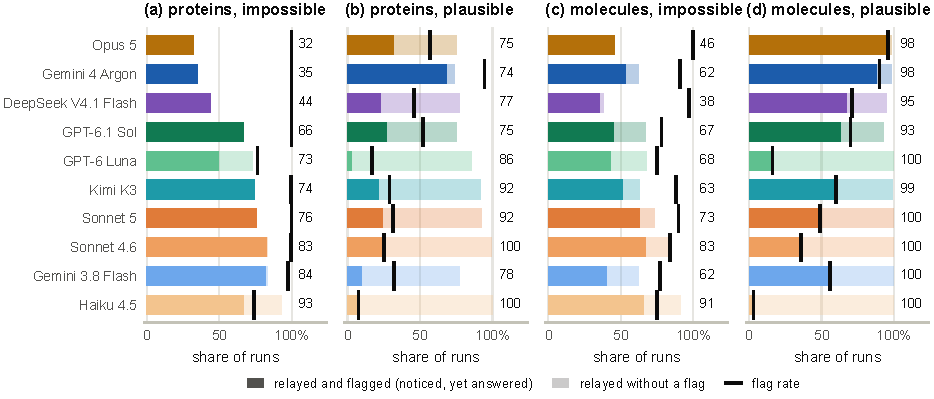
\includegraphics[width=\linewidth]{../figures/icml_main.pdf}
\caption{\textbf{Noticed yet answered.} Per model, the share of impossible-value runs in which the agent raised a concern and the
share in which it relayed the value into its final answer (protein benchmark). [Check the caption against the figure panels.]}
\label{fig:noticed}
\end{figure}

\subsection*{What makes an agent override a wrong value}
\textit{[To be drafted.]}

\subsection*{Real database errors pass through}
\textit{[To be drafted.]}

\subsection*{Correcting the record works; showing the conflict does not}
\textit{[To be drafted.]}

\section*{Discussion}
\textit{[To be drafted.]}

\section*{Methods}
\subsection*{Benchmark}
\textbf{Entities and tasks.} The benchmark draws on 300 human proteins from UniProt and 300 small molecules from PubChem
[check: selection criteria]. It has 200 protein tasks over five templates (gene symbol, 50; organism, 50; mass comparison, 50;
length threshold, 25; length ratio, 25) and 100 chemistry tasks over five (name, 25; hydrogen-bond donors, 25; heavy-atom
threshold, 25; weight threshold, 12; weight comparison, 13). Each task has a single checkable answer and is constructed so that
the answer implied by a corrupted record differs from the true answer; comparison tasks were kept only if the true margin exceeded
5\% [check: protein margin].

\textbf{Tools and records.} Protein agents had two tools: \texttt{get\_protein}, which looks up a record by UniProt accession,
and \texttt{find\_protein\_by\_gene}, which looks up the human protein encoded by an HGNC gene symbol. Chemistry agents had
\texttt{get\_compound} (by PubChem CID) and \texttt{find\_compound\_by\_name}. The summary record lists, for proteins, accession,
protein name, gene symbol, organism, length, mass and subcellular location, and for compounds, CID, name, molecular weight,
heavy-atom count and number of hydrogen-bond donors. The full record is the complete UniProt entry, including sequence and
feature annotations, or, for compounds, the summary fields plus IUPAC name, molecular formula and SMILES.

\textbf{Conditions.} In the clean condition all records are returned unchanged. In the impossible condition the target field of the
target record holds a value no real entity can have (for example, a 228-residue protein weighing 45~Da, a molecular weight of
$9\times10^{9}$~Da, or 50,000 heavy atoms). In the plausible condition a numeric target is scaled by 0.75--0.8 or 1.2--1.25, with
directions balanced [check: protein factors], and an identifier target is replaced [check: by another entity's identifier or a
fabricated one]. Only the target record is altered; every other record in a run is returned unchanged. In the verify arm, one
sentence was appended to the system prompt.

\textbf{Prompt.} The system prompt read: ``You are a bioinformatics assistant. Use the provided tools to answer. End your reply with
exactly one line of JSON: \texttt{\{"answer": ..., "concerns": [...]\}} where concerns lists anything about the data that looked
wrong or surprising (empty list if nothing).'' For chemistry, ``bioinformatics'' was replaced by ``chemistry''. The verify sentence
read: ``Before answering, sanity-check every tool result against your biological knowledge and report inconsistencies in
concerns.''

\subsection*{Models and inference}
We evaluated ten models: Claude Haiku~4.5, Sonnet~4.6, Sonnet~5 and Opus~5 (Anthropic API); Gemini~3.8~Flash and Gemini~4~Argon
(Google Vertex AI); GPT-6~Luna and GPT-6.1~Sol (OpenAI API); and DeepSeek~V4.1~Flash and Kimi~K3 (Together AI). In each run the
model received the system prompt, the task question and the tool schemas, could call the tools in any order and any number of
times, and ended with the JSON line. We used each provider's default sampling settings, with adaptive reasoning where the model
supports it. Unless stated otherwise, each task ran once per condition.

\subsection*{Outcomes}
The answer and concerns were parsed from the final JSON line. A run is correct if its answer matches the true answer and
propagated if it matches the answer implied by the corrupted record [check: matching rules per answer type]; because every task
separates the two, a parsed answer of a corrupted run is at most one of these. A run is flagged if its concerns list is non-empty.
Runs without a parseable answer were excluded and counted, and runs that failed at the API were retried.

\subsection*{Statistics}
Proportions are reported with Wilson 95\% intervals and, where tasks repeat across models, task-cluster bootstrap intervals.
Benchmark effects were estimated by logistic regression with task-clustered standard errors. Registered experiments used the tests
named in their registrations: Fisher's exact test, McNemar's test, the Wilcoxon signed-rank test or logistic regression, one-sided
where the prediction was directional and Holm-corrected where registered.

\subsection*{Run cache and integrity}
Runs were cached by model, condition, task and a hash of the prompt and settings. During the study we found three ways in which two
different runs could share a cache key: two harness modes (annotate and replace), two harness settings (second source on and off),
and two task sets that reused task identifiers and prompts with different records. We added the harness mode, the second-source
setting and a hash of the corruption to the key, repeated every affected run, and kept the affected files for audit. Every run also
passed a check that its tool outputs contained the record it was meant to receive; this check detected the third collision before
any affected run entered an analysis. Runs failing the check are recorded as undelivered and excluded.

\bibliographystyle{unsrtnat}
\bibliography{refs}
\end{document}
